\documentclass[12pt]{article}
\usepackage{pictex,fancyhdr}
\usepackage{amsmath,amsfonts,amsbsy}
\usepackage{fullpage}
\usepackage{graphicx}

\begin{document}
\subsection{Ex7:}
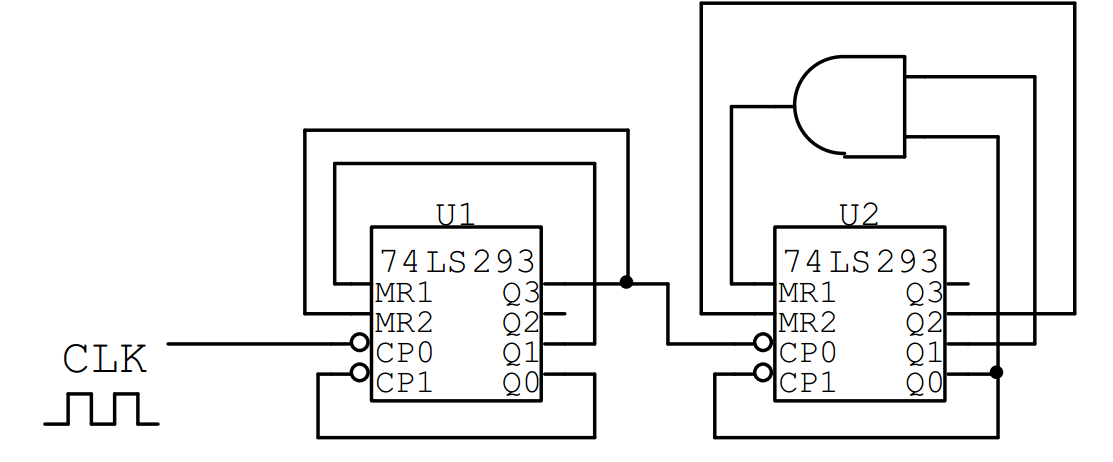
\includegraphics[scale = 0.7]{hinh1.png}
\bigbreak
- The frequency of the clock signal is $f_{CLK}$ = 35KHz. \\
\begin{enumerate}
	%1
	\item What is the MOD of the counter ? \\
	- This is MOD-70 counter.
	\begin{itemize}
		\item The circuit consists of 2 IC asynchronous counter.
		\item The first IC (U1) is MOD-10 counter.
		\item The second IC (U2) is MOD-7 counter.
	\end{itemize}
	%2
	\item Determine the frequency of Q3 of U1:
	- The frequency of Q3: \\
	\begin{center}
		$f_{Q3} = \dfrac{f_{in}}{10} = \dfrac{35 \times 10^{3}}{10} = 3500$ (Hz)
	\end{center}
	%3
	\item Determine the frequency of Q2 of U2:
	- The frequency of Q2: \\
	\begin{center}
		$f_{Q2} = \dfrac{f_{in}}{70} = \dfrac{35 \times 10^{3}}{70} = 500$ (Hz)
	\end{center}
	%4
	\item In the Q3, Q2, Q1, Q0 signals of U1 and U2, which signals are glitches ? \\
	- In U1, Q1 and Q3 is glitches. \\
	- In U2, Q2, Q0 and Q1 is glitches. \\
	%5
	\item Determine the duty circle of Q2: \\
	\begin{center}
		$T_{Q2} = \dfrac{1}{f_{Q2}} = \dfrac{1}{500} = 2 \times 10_{-3}$ (s)
	\end{center}
\end{enumerate}
\end{document}
 